\documentclass{beamer}
\usetheme{Madrid}
\usecolortheme{default}
\usepackage[utf8]{inputenc}
\usepackage[spanish]{babel}
\usepackage{amsmath, amssymb}
\usepackage{graphicx}

\setbeamertemplate{headline}{
  \leavevmode%
  \hbox{% 
  \begin{beamercolorbox}[wd=.5\paperwidth,ht=2.5ex,dp=1ex,left]{section in head/foot}%
    \hspace{1em}\textbf{M\'etodos de Optimizaci\'on}
  \end{beamercolorbox}%
  \begin{beamercolorbox}[wd=.5\paperwidth,ht=2.5ex,dp=1ex,right]{section in head/foot}%
    \textbf{Universidad Nacional del Altiplano - FINESI}\hspace{1em}
  \end{beamercolorbox}}%
}

\setbeamertemplate{footline}[frame number]

\title{Universidad Nacional del Altiplano Puno}
\subtitle{Escuela Profesional de Ingenier\'ia Estad\'istica e Inform\'atica}

\author{
  \textbf{Modelo programación lineal para minimizar los costos de producción de una empresa de cintas adhesivas} \\
  \vspace{0.5cm}
  \textbf{Profesor:} \\
  Fred Torres Cruz \\
  \\
  \textbf{Presentado por:} \\
  Belinda paza Quispe
}

\institute{}

\date{07 de mayo del 2025}

\begin{document}

\begin{frame}
  \titlepage
\end{frame}

\begin{frame}{Introduccion}
  \textbf{Identificación del problema:} \\
  El estudio partio de una situaion en una empresa de Colombia que fabrica cintas adhesivas, la cual esta empresa enfrentaba altos costos de produccion debido a la planificacion de produccion poco eficiente.
  El objetivo era encontrar una forma de minimizar los costos totales de produccion, considerando diversos factores como:
  \begin{itemize}
    \item Costos de materias primas
    \item Costos de mano de obra directa
    \item Costos de almacenamiento e inventario
    \item Costos por cambios de línea (setup)
    \item Capacidad de las máquinas
  \end{itemize}
\end{frame}

\begin{frame}{Metodolog\'ia}
\small
  \textbf{Metodologia aplicada:} \\
  Se desarrollo una metodologia en dos fases:
  \begin{itemize}
    \item \textbf{Fase 1:} Descomposicion del problema mediante unamatriz de incidencia, el cual permitio dividir el problema general en subproblemas.
    \item \textbf{Fase 2:} Formulacion y aplicacion de un modelo de programacion lineal para cada subproblema, con el fin de determinar los tamaños optimos de lote de produccion que minimicen los costos.
  \end{itemize}
  \begin{center}
    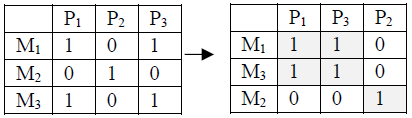
\includegraphics[width=0.50\linewidth]{Captura de pantalla 2025-05-07 003257.png}
  \end{center}
\end{frame}





\begin{frame}{Modelo Matem\'atico}
\footnotesize
  \textbf{Funcion objetivo:} \\
  Minimizar el costo total de producción.
  Esto incluye:
  \begin{itemize}
    \item Costos de produccion
    \item Costos de inventario
    \item Costos de no satisfacer demanda 
    \item Costos de setup
  \end{itemize}
{\footnotesize
\[ \min Z = \sum_{i,m,t} C_{\text{PROD}}(i,m) X_{imt} + \sum_{i,t} CI(i) I_{it} + \sum_{i,t} B(i) F_{it} + \sum_{i,m,t} CS(i,m) y_{imt} \]
}
  \textbf{Variables de decisión:} \\
  Representan la cantidad a producir de cada producto dentro de cada grupo.
  \textbf{Restricciones:} \\
  \begin{itemize}
    \item Balance de inventario
    \item tiempo de produccion
    \item Inventario de seguridad 
    \item Binaria (se produce o no); (1, 0)
  \end{itemize}\\
\end{frame}

\begin{frame}{Implementacion}
  \begin{columns}
    \begin{column}{0.55\textwidth}
      \textbf{Implementacion en la empresa:} \\
      Se inició con el cálculo de pronósticos con la herramienta Statgraphics. Resultaron 6 pronósticos para cada una.\\
      Luego se realizo la matriz de incidencia para identificar compatibilidad de las máquinas, y la generación de subproblemas.
    \end{column}
    \begin{column}{0.45\textwidth}
      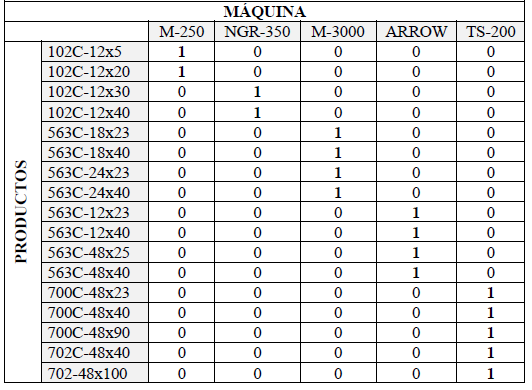
\includegraphics[width=\linewidth]{Captura de pantalla 2025-05-07 012246.png}
    \end{column}
  \end{columns}
\end{frame}


\begin{frame}{Programacion lineal}
\footnotesize
  Para la obtención de los datos de entrada fue necesario que las unidades del modelo de programación lineal se definieran en bajadas de producción.\\
  Se definió que los datos de entrada serian:
\begin{itemize}
  \item Costos unitarios: (producci\'on, setup, inventario, faltante)
  \item Tiempos: (setup, producci\'on)
  \item Inventarios iniciales
\end{itemize}
\textbf{ } \\
  Luego fueron calculados los diferentes costos que se ingresaron en el modelo de Programacion Lineal ya que cada uno trata con su propio modelo de programacion lineal.

\textbf{Resultados: } \\
El modelo fue validado con resultafos positivos, ya que al hacer la comparacion entre el costo real al costo del modelo, el cual los costos proyectados por el modelo fueron inferiores a los costos reales. \\
\begin{tabular}{lcc}\\
\textbf{Subgrupo} & \textbf{Costo Real} & \textbf{Costo Modelo (Z)} \\
1 & \$55M & \$38M (\textbf{-30\%}) \\
2 & \$37M & \$31M (\textbf{-14\%}) \\
3 & \$148M & \$114M (\textbf{-22\%}) \\
4 & \$270M & \$224M (\textbf{-17\%}) \\
5 & \$475M & \$269M (\textbf{-43\%}) \\
\end{tabular}
\end{frame}


\end{document}
